\section{ SR02US22 }


\subsection{Meta}

    \textbf{Title:}
    Current Trends in Operating Room Scheduling 2015 to 2020: a Literature Review

    \begin{table}[H]
        \centering
        \begin{tabular}{|c|c|c|c|c|c|c|c|c|}
            \hline
                \textbf{Rank} & \textbf{Grasp} & \textbf{Type} & \textbf{Outcome} & \textbf{Domain} & \textbf{COV19} & \textbf{CoI} & \textbf{DB} & \textbf{Prooved} \\
            \hline
                5 & 95\% & A & P & S & No & No & Has & Yes \\
            \hline
        \end{tabular}
        \caption{Reference's metadata}
        \label{tab:SR02US22}
    \end{table}

\subsection{Summary}
Sean Harris and David Claudio \cite{x079} conducted literature on current operating room scheduling trends from 2015 to 2020. This literature review updates knowledge about new studies continuing the three previous reviews. The authors also introduced new categories and metrics for structuring and analysing the findings. The categories were evaluated individually by complexity criteria, and at the end, the collective average complexity of the research works was presented. The research focuses mainly on the Operating Room Scheduling problem and less on the proposed solutions. Sean Harris and David Claudio underline the most promising future scheduler development directions. The emphasis is placed on the geographic location for the generalisation research and on the need for more practical implementations of the scheduling models.


\subsection{Notes}
    \begin{itemize}
        \item Cascade of literature reviews from 2000 to 2020;
        \item The geographical location by hospital or the first affiliation;
        \item Models generalisation from one country to another (urban to rural);
        \item Leeftink and Hans (153) dataset;
        \item Systematic texting and validation (32, 19, 230)
        \item Look into the next studies: 1, 8, 12, 231, 262;
        \item (thoughts) statistics by researchers in the fiel; 
        \item (thoughts) geographical locations by countries and/ or cities;
    \end{itemize}


\subsection{Reading}
    
    
    \textbf{Page 1:}
    The abstract presents the papers as literature review based on the previous review studies in the field of operating room (OR) scheduling up to 2014. The current paper reviews 246 from 2015 to 2020 and underlines the next tengencies: the number of publications has grown in comparison with brevious years, the development continues across all categories, and there is still unsufficient number of practical implementations of the schedulers. OT is the most valuable financial asset in hospitals, and it is possible to solve the OT scheduling problem from multiple approaches.
    
    \textbf{Page 2:}
    There is multiple benefits from conducting a literature review: organise available materials, points towart uncharted teritories, and provides common guidance for newcommers. The current literature review is build upon three previous reviews by followinf classification, but there are some works which does not follow the framed classifications.
    
    \textbf{Page 3:}
    There are further extentions of the classification system: +location, +OR research frequency, two new subcategories in waiting time constraint, +planning horison, +scheduling policy
    \begin{figure}[H]
        \centering
        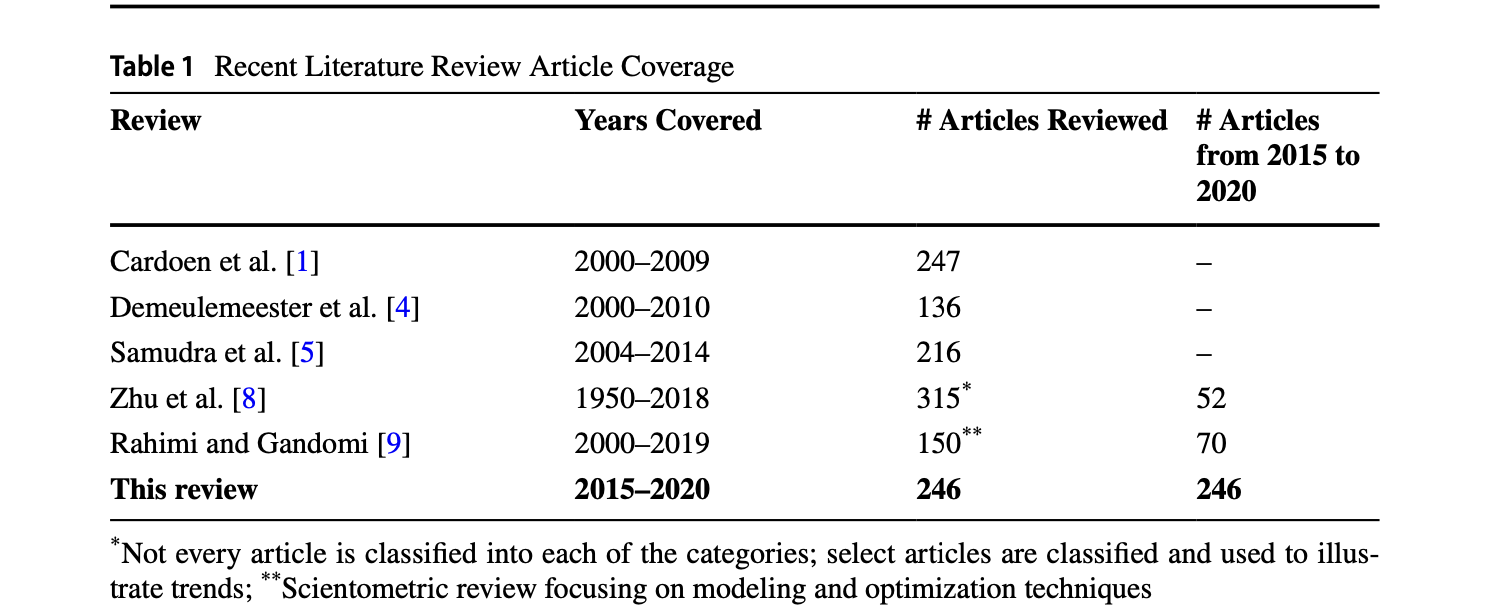
\includegraphics[width=1\textwidth]{figures/0002_SR02US22/fig1.png}
        \caption{Previous literature reviews from \cite{x079}.}
        \label{fig1:SR02US22}
    \end{figure}
    
    \textbf{Page 4:}
    There is replicated search strategy from the previous literature review considering only English and two major databases Web of Science and PubMed.
    \begin{figure}[H]
        \centering
        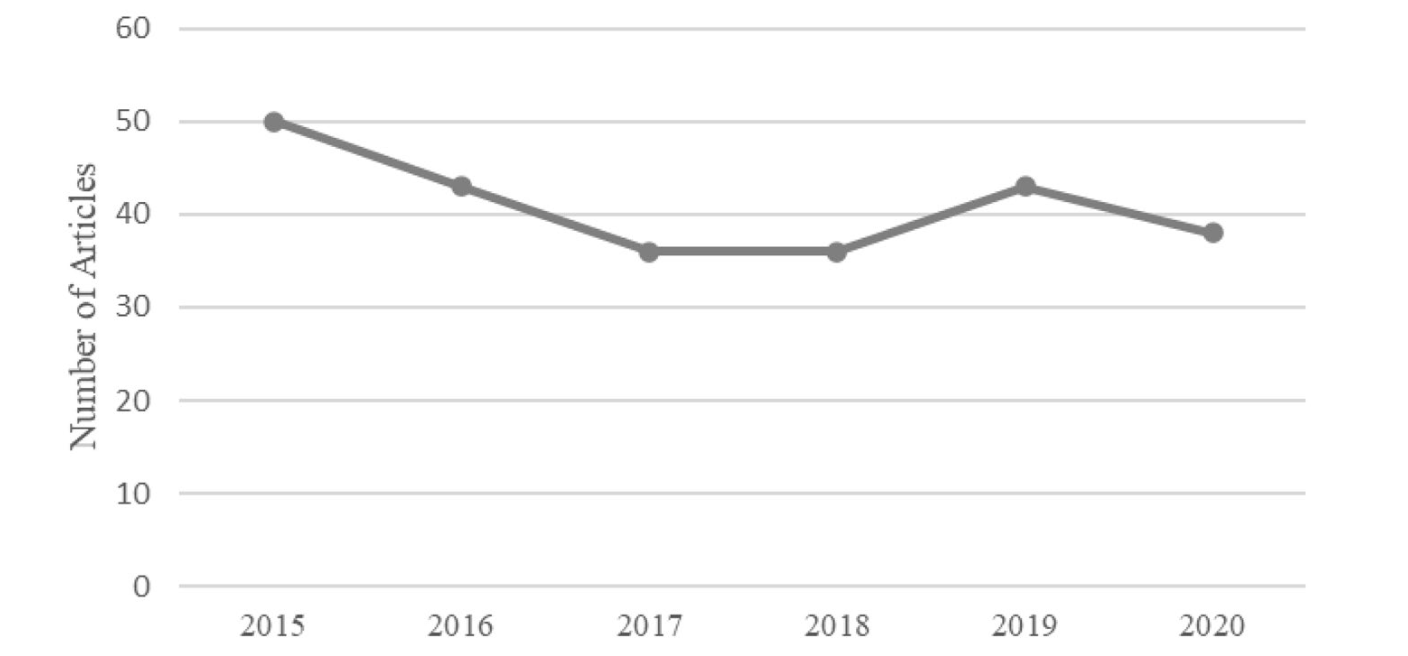
\includegraphics[width=1\textwidth]{figures/0002_SR02US22/fig2.png}
        \caption{Number of articles per year \cite{x079}.}
        \label{fig2:SR02US22}
    \end{figure}
    
    \textbf{Page 5:}
    Sean Harris and David Claudio introduces complexity score for every category. Patients classification of elective and non-elective, inpatients and outpatients. If models do not use in-/outpatients classification then it is classified as general elective case. Non-elective cases can be categorised as emergent (up to 1 hour), urgent (up to 1 day), or general. 241 of 246 papers consider elective cases alone. From 2015 to 2020 the number of papers with clear separation of outpatients and inpatients decreased. Non-elective patient is a challenge for scheduling.

    \textbf{Page 6:}
    There are two solutions to emergent cases: just go ahead with emergent-first; brack-in method (231). Proper schedulers evaluation is not possible due to abcense of general scheduling policy.
    Dedicated, shared, and hybrid OR policies are considered for non-elective cases. 
    
    \textbf{Page 7:}
    Most researchers assume that there is dedicated emergent OR. The patient's complexity scores 1 is there is elective and non-elective cases and 0 otherwise. The OR policies is still a debatable topic.
    
    \textbf{Page 8:}
    There are divarse objectives for each of the partisipance in healthcare services: patients, stakeholders, managers, and medical personnel. Two new terms: \underline{waiting time-number of days} and \underline{waiting time-within day}. Financial objectives are usually competing (cancellation $<->$ overtime). Overtime not always mean overutilisation. And oferal performance values have been improved from 2015 to 2020.
    
    \textbf{Page 9:}
    Some constraint measures are more likely to be selected with one another than others which is visulised in tables. Complexity scrore for two objectives is 0.5 and for more than two objectives - 1. There are positive trends in direction of staff sutisfaction.
    
    \textbf{Page 10:}
    The authors state that the number of objective measurment will increase in future studies. The next three decision levels are usually considered: Case-mix planning (strategic = long), master Surgery planning (MSP = MSS = tactical = medium = 1 week), Patient scheduling (operational = short). In addition, there are three scheduling policies: block (allocation scheduling = defining start time), open (FIFO = FCFS), and modified block. The alternative way of analysing the decision aspect of the scheduling is by specialty, surgeon, and patient. The most popular is still patient-level panning. 
    
    \textbf{Page 11:}
    There are papers which considere multiple levels of decision-making at once (12, 262). Some exotic works propose solutions for OR scheduling problem and vehicle routine problem. The various planning horisons are picked for scheduling includion varying horisons.

    \textbf{Page 12:}
    The planning horizon is not always assigned explisitaly. Some researchers work on dynamic scheduling but many more on rescheduling strategies which allows have idea of required capacity on weeks ahead and then more concreat scheduling in one/ two days prior to the surgery day.
    
    \textbf{Page 13:}
    Additinonal diration is online scheduling (on-the-fly desicon-making). There is developed terminology by (1) which is good to follow.
    
    \textbf{Page 14:}
    Upstream/ Downstream Units introduce new level of complexity to the scheduling model: hardship to generalise the research and increase scheduling time, but rewards with more applicability of the solution. From 2000 to 2014 around 50\% of papers studies include at least one of the units. Most researchers select downstream unit over upstream. Medical equipment as well as sterilization processing department became popular objectives of the scheduling problem.
    
    \textbf{Page 15:}
    The ICU models are unpredictable, thus use stochastic approaches. Incorporating turnover time is a usual practice. The authros sugest increase in investigation uncommon upstream and downstream units.

    \textbf{Page 16:}
    In general, from 50\% to 60\% of studies incorporate uncertainties. The most common is operation duration with is good trend that should remain. Sean Harris and David Claudio also suggest to improve research in the area of rescheduling. The solution methods are ordered by frequency: mathematical models, simulation approaches, methaheuristics (60\%-30\%~23\%).

    \textbf{Page 16:}
    The research methods are not easaly classified. The heuristics reduce scheduling time in cost of 0 to 10\% of optimality gap.
    
    \textbf{Page 17:}
    In the gap between 2015 and 2020 the papers with simulation optimisation solutions begone to appear. MIP $->$ goal programming. Simulation optimisation, hybrit simulation, heuristics, and goal programming are promissing and suggested scheduling approaches.
    
    \textbf{Page 18:}
    Future reviews should adress the scheduling methods classifications. Healthcare requires practical validation of the scheduler work. The use of real data increased to 7\% which showcases the increase and availability of healthcare records and enphacise the vast room for imptovement.
    
    \textbf{Page 19:}
    The number of implemented models from 2015 to 2020 is reduced. The level of details in research workflow is increased and the investigators benefit from interviews with medical personnel.
    
    \textbf{Page 20:}
    Systematic texting and validation (32, 19, 230).
    \begin{figure}[H]
        \centering
        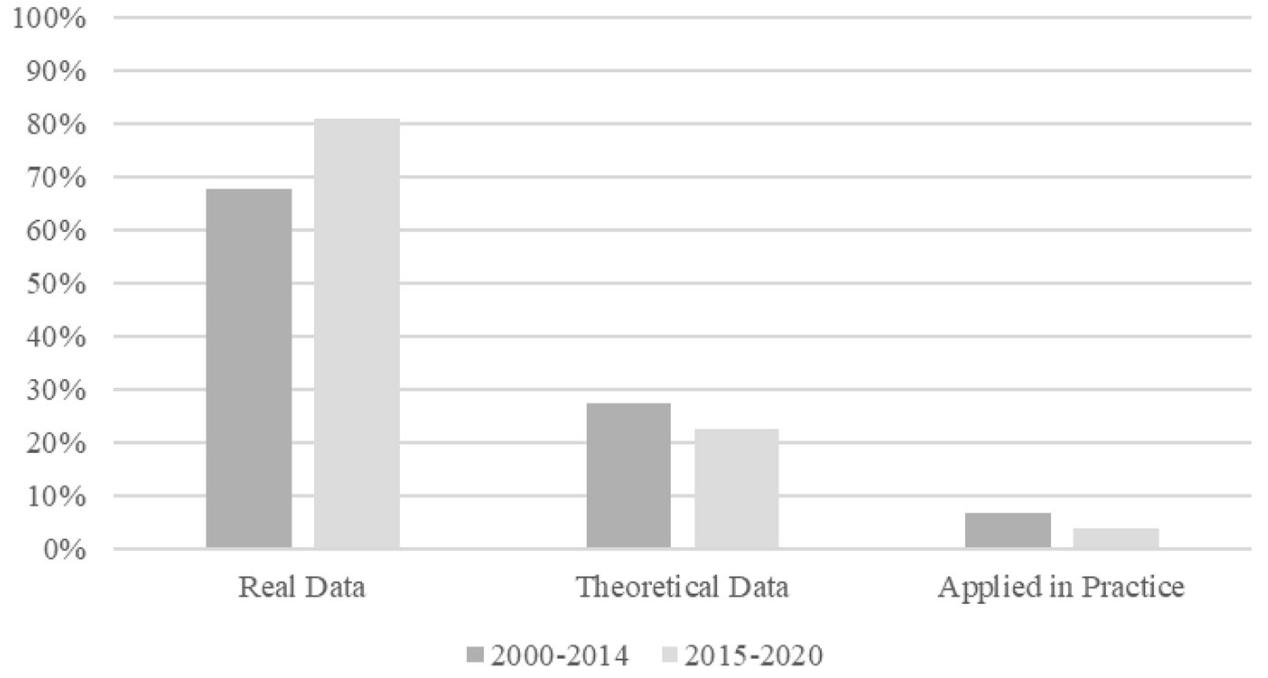
\includegraphics[width=.8\textwidth]{figures/0002_SR02US22/fig3.png}
        \caption{Testing and application from \cite{x079}.}
        \label{fig3:SR02US22}
    \end{figure}

    \textbf{Page 21:}
    Future is in generalisable findings. Location critaria is taken into account for studies with real data (Leeftink and Hans (153) does not count). USA and China are the most common origins of the OR scheduling research. Most of US is in Mayo Clinic or the Northeastern and Midwestern part of the country. In Europe the lieading position is in Italy.
    
    \textbf{Page 22:}
    Using location cretatio opens new perspective in the literature review analysis.
    \begin{figure}[H]
        \centering
        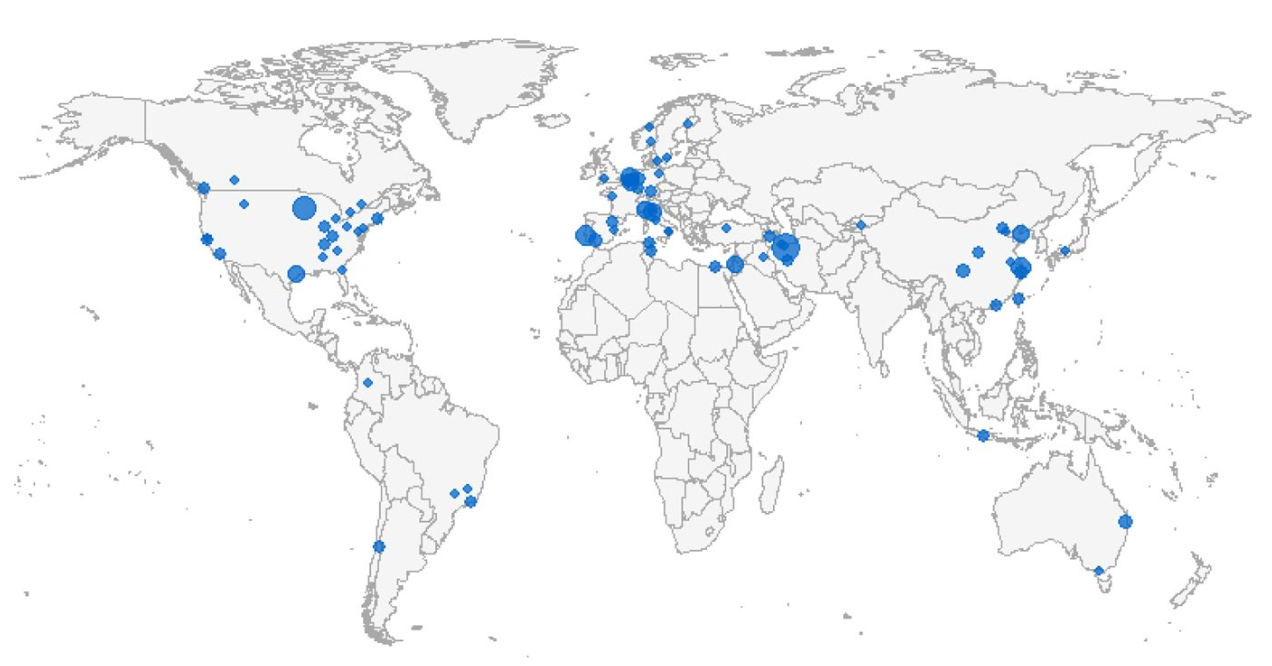
\includegraphics[width=1\textwidth]{figures/0002_SR02US22/fig4.png}
        \caption{Geographic Map of Article Locations and Frequency from \cite{x079}.}
        \label{fig4:SR02US22}
    \end{figure}
    \begin{figure}[H]
        \centering
        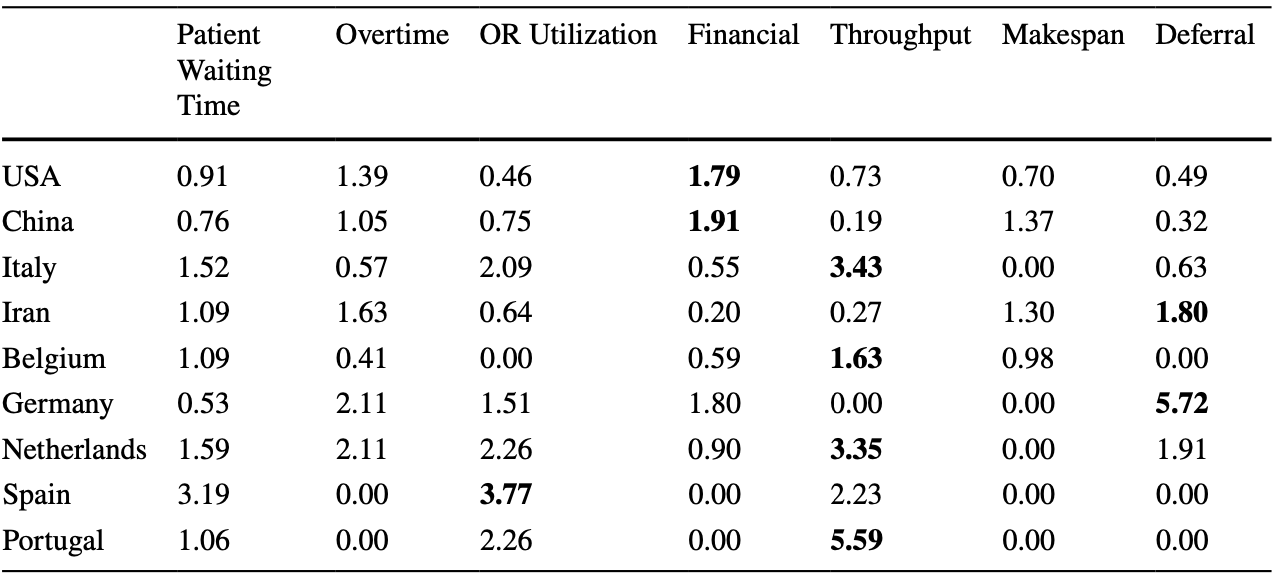
\includegraphics[width=1\textwidth]{figures/0002_SR02US22/fig5.png}
        \caption{Ratio of Actual/Expected Occurrence of PM by Country from \cite{x079}.}
        \label{fig5:SR02US22}
    \end{figure}
    
    \textbf{Conclusions:}
    Review on 246 studies from 2015 to 2020 was conducted. \underline{Patient type} is consistant and future works are in direction of non-elective cases (centralised vs. deventralised). The tendency of multiple \underline{performance measures} should continue. All \underline{decision delineations} (dynamic scheduling, rescheduling and online scheduling) are continuing to be desirable areas of research. The \underline{not traditional upstream capacities} could be considered for future research. Incorporating more \underline{uncertainty} in OR schedulers. \underline{Research methodology} lies in development of heuristics and the suggestion areas are simulation-optimisation and goal programming. More research is needed in \underline{testing and application}. Innovative diraction is to consider generalisation from one \underline{geographic location} to another. For the papers in the research the complexity score increases closer to 2020. The collective work shows its benefits, but the field remains scarce meaning the challeges are not easy to concore.